\documentclass[tikz]{standalone}
\usepackage{pgfplots}
\pgfplotsset{compat=1.17}

\begin{document}
  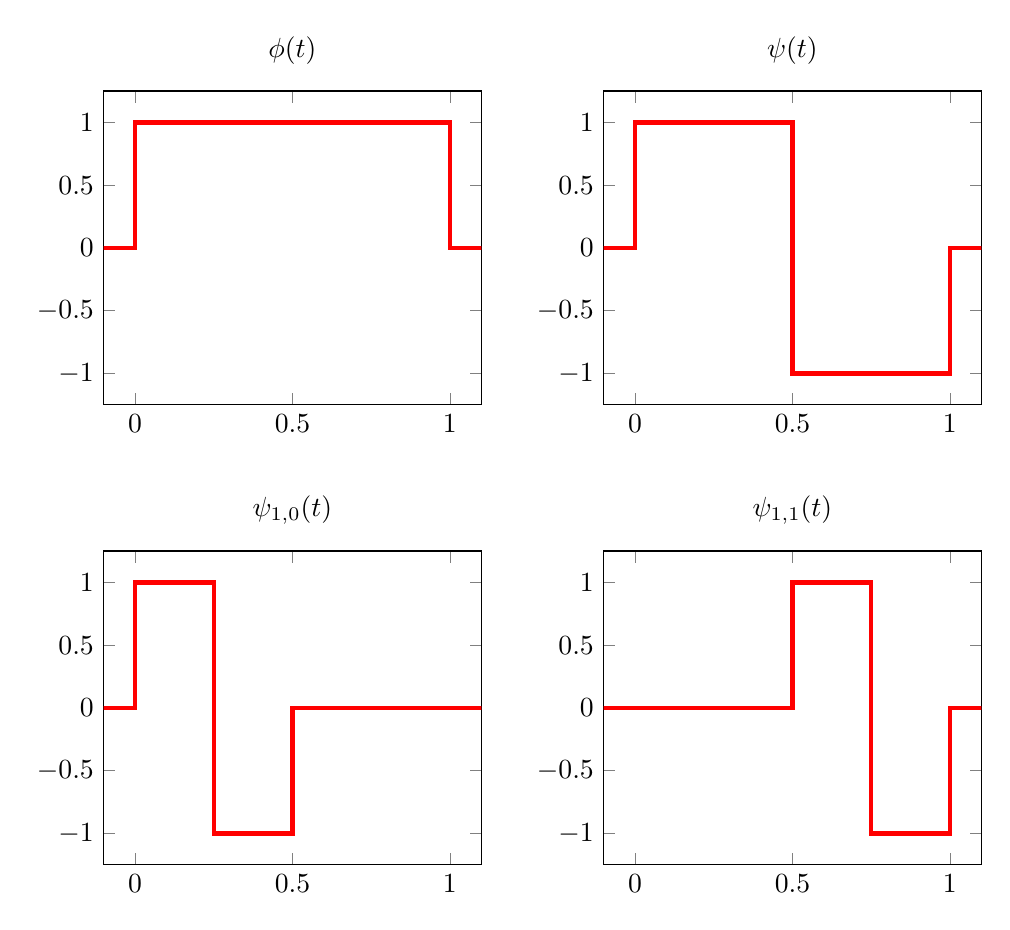
\begin{tikzpicture}
    \begin{scope}
      \begin{axis}[scale=.7, title={$\phi(t)$},
        xmin = -.1, xmax = 1.1,
        ymin = -1.25, ymax = 1.25,
        xtick = {0,1/2,1},
        ytick = {-1,-1/2,0,1/2,1},
        ]
        \addplot[mark=none,ultra thick,red] coordinates {
          (-1,0)
          (0,0)
          (0,1) 
          (1,1)
          (1,0)
          (2,0)
          };
      \end{axis}
    \end{scope}
    \begin{scope}[xshift=2.5in]
      \begin{axis}[scale=.7, title={$\psi(t)$},
        xmin = -.1, xmax = 1.1,
        ymin = -1.25, ymax = 1.25,
        xtick = {0,1/2,1},
        ytick = {-1,-1/2,0,1/2,1},
        ]
        \addplot[mark=none,ultra thick,red] coordinates {
          (-1,0)
          (0,0)
          (0,1) 
          (1/2,1)
          (1/2,-1)
          (1,-1)
          (1,0)
          (2,0)
          };
      \end{axis}
    \end{scope}
    \begin{scope}[yshift=-2.3in]
      \begin{axis}[scale=.7, title={$\psi_{1,0}(t)$},
        xmin = -.1, xmax = 1.1,
        ymin = -1.25, ymax = 1.25,
        xtick = {0,1/2,1},
        ytick = {-1,-1/2,0,1/2,1},
        ]
        \addplot[mark=none,ultra thick,red] coordinates {
          (-1,0)
          (0,0)
          (0,1)
          (1/4,1)
          (1/4,-1)
          (1/2,-1)
          (1/2,0)
          (2,0)
          };
      \end{axis}
    \end{scope}
    \begin{scope}[xshift=2.5in,yshift=-2.3in]
      \begin{axis}[scale=.7, title={$\psi_{1,1}(t)$},
        xmin = -.1, xmax = 1.1,
        ymin = -1.25, ymax = 1.25,
        xtick = {0,1/2,1},
        ytick = {-1,-1/2,0,1/2,1},
        ]
        \addplot[mark=none,ultra thick,red] coordinates {
          (-1,0)
          (1/2,0)
          (1/2,1)
          (3/4,1)
          (3/4,-1)
          (1,-1)
          (1,0)
          (2,0)
          };
      \end{axis}
    \end{scope}
  \end{tikzpicture}
\end{document}